\documentclass{article}
\usepackage{amsmath}
\usepackage{amssymb}
\usepackage{graphicx}
\usepackage[font=scriptsize,labelfont={bf}]{caption}
\usepackage[justification=raggedright,nearskip=10pt,farskip=0pt]{subfig}%[FIGTOPCAP, raggedright, hang, nooneline]{subfigure}
%\usepackage{subfig}
\usepackage{calc}
\usepackage{url}
\usepackage{array}
\usepackage{rotating}
\usepackage{tabularx}
%\usepackage{wasysym}
\usepackage{multirow}
%\usepackage[title]{appendix}
%\usepackage[authoryear]{natbib}
%\usepackage{cite}
%\usepackage{named}
%\usepackage{setspace}
\usepackage{layouts}
%\usepackage{titlesec}
%\usepackage[multiple]{footmisc}
%\usepackage{enumitem}
\usepackage{titletoc}
\usepackage{setspace}
\usepackage{longtable}

\hbadness=9999999 %avoid complaining for underfull h/vbox
\vbadness=9999999

% \setlength{\columnwidth}{86mm}
 \captionsetup[subfloat]{position=top, justification=raggedright, singlelinecheck=false, labelformat=simple, font={scriptsize,sf,bf}}
 \renewcommand*\thesubfigure{\Alph{subfigure}}
 \setlength{\belowcaptionskip}{-3mm}
 %\setlength{\abovecaptionskip}{0mm}
%\addtolength{\abovecaptionskip}{-3mm}

%\subfiguretopcaptrue

\pdfminorversion=4
\pdfobjcompresslevel=0

\usepackage{pgf}
\usepackage{tikz}
\usetikzlibrary{shapes,arrows}

\usepackage{footnote}

\pgfdeclareimage[width=13.9cm]{animo-logo}{images/animo_logo}
\pgfdeclareimage[height=3ex]{win-logo}{images/win_logo}
\pgfdeclareimage[height=3ex]{mac-logo}{images/mac_logo}
\pgfdeclareimage[height=3ex]{linux-logo}{images/linux_logo}
\pgfdeclareimage[height=3ex]{ubuntu-logo}{images/ubuntu_logo}
\pgfdeclareimage[height=2ex]{mac-command}{images/mac_command}
\pgfdeclareimage[height=1.5ex]{contact-email}{images/email}

\newcommand{\winsymbol}{\raisebox{-0.8ex}{\pgfuseimage{win-logo}}}
\newcommand{\macsymbol}{\raisebox{-0.5ex}{\pgfuseimage{mac-logo}}}
\newcommand{\linuxsymbol}{\raisebox{-0.8ex}{\pgfuseimage{linux-logo}}}
\newcommand{\ubuntusymbol}{\raisebox{-0.9ex}{\pgfuseimage{ubuntu-logo}}}
\newcommand{\winmaclinux}[3]{\begin{itemize}
    \item[\winsymbol] #1
    \item[\macsymbol] #2
    \item[\linuxsymbol] #3
\end{itemize}}
\newcommand{\macpc}[2]{\begin{itemize}
    \item[\macsymbol] #1
    \item[\winsymbol\ \  \linuxsymbol] #2
\end{itemize}}
\newcommand{\winandmacorlinux}[2]{\begin{itemize}
    \item[\winsymbol\ \  \macsymbol] #1
    \item[\linuxsymbol] #2
\end{itemize}}

\newcommand{\maccmd}{\raisebox{-0.35ex}{\pgfuseimage{mac-command}}}

\newcommand{\contactemail}{\pgfuseimage{contact-email}}

\setlength{\abovecaptionskip}{1.3mm}
%\setlength{\belowcaptionskip}{1mm}

\def\ta{Timed Automaton}
\def\tas{Timed Automata}

% \setlength{\oddsidemargin}{1.875in}
% \setlength{\evensidemargin}{1.875in}
% \addtolength{\textwidth}{-3.75in}

\newlength\addedmarginsingle
\setlength\addedmarginsingle{-0.6in}
\newlength\addedmargintotal
\setlength\addedmargintotal{2\addedmarginsingle}

\addtolength{\oddsidemargin}{\addedmarginsingle}
\addtolength{\evensidemargin}{\addedmarginsingle}
\addtolength{\textwidth}{-\addedmargintotal}
\addtolength{\linewidth}{-\addedmargintotal}
\addtolength{\hsize}{-\addedmargintotal}
\addtolength{\topmargin}{\addedmarginsingle}
\addtolength{\textheight}{-\addedmargintotal}
\addtolength{\vsize}{-\addedmargintotal}

\begin{document}

\pagestyle{plain}

\clearpage
% \thispagestyle{empty}\ \

\thispagestyle{empty}
\ \\ \ \\ \ \\ \ \\ \ \\
\begin{center}
 %{\Huge Bringing biological networks}\\ \ \\ {\Huge to life with ANIMO}\\ \ \\ \ \\
  \pgfuseimage{animo-logo}\\ 
  {\huge\sf Analysis of Networks with Interactive MOdelling}\\\ \\ \ \\ \ \\ \ \\
 {\Huge User's Manual}
\end{center}
\clearpage






\makeatletter

% Copied from the LaTeX sources
\def\addcontentsline#1#2#3{%
  \addtocontents{#1}{\protect\contentsline{#2}{#3}{\thepage}}}
\long\def\addtocontents#1#2{%
  \protected@write\@auxout
    {\let\label\@gobble \let\index\@gobble \let\glossary\@gobble}%
    {\string\@writefile{#1}{#2}}}
\titlecontents{section} % set formatting for \section -
                        % \subsection must be formatted separately
[2.em]                 % adjust left margin
{\bf}             % font formatting
{\contentslabel{2.em}} % section label and offset
{\hspace*{-2.em}}
{\titlerule*[1pc]{}\contentspage}
\titlecontents{subsection} % set formatting for \section -
                        % \subsection must be formatted separately
[4.5em]                 % adjust left margin
{\rmfamily}             % font formatting
{\contentslabel{2.5em}} % section label and offset
{\hspace*{2.5em}}
{\titlerule*[1pc]{.}\contentspage}
% Copied from article.cls
%\setcounter{tocdepth}{5}
\renewcommand\tableofcontents{%
\begin{spacing}{1.3}
    \section*{\contentsname
        \@mkboth{%
           \MakeUppercase\contentsname}{\MakeUppercase\contentsname}}%
    \@starttoc{toc}%
\end{spacing}
}
% \newcommand*\l@paragraph{\@dottedtocline{4}{7.0em}{4.1em}}
% \newcommand*\l@subparagraph{\@dottedtocline{5}{10em}{5em}}
% \newcommand\listoffigures{%
%     \section*{\listfigurename}%
%       \@mkboth{\MakeUppercase\listfigurename}%
%               {\MakeUppercase\listfigurename}%
%     \@starttoc{lof}%
%     }
% \newcommand*\l@figure{\@dottedtocline{1}{1.5em}{2.3em}}
% \newcommand\listoftables{%
%     \section*{\listtablename}%
%       \@mkboth{%
%           \MakeUppercase\listtablename}%
%          {\MakeUppercase\listtablename}%
%     \@starttoc{lot}%
%     }
% \let\l@table\l@figure

\makeatother




\addtocontents{toc}{\protect\setcounter{tocdepth}{5}}
\thispagestyle{empty}
\tableofcontents
\clearpage

\setcounter{page}{1}
\setcounter{section}{0}

\renewcommand\figurename{Figure}
% \renewcommand*\thefigure{S\arabic{figure}}
% \renewcommand*\thetable{S\arabic{table}}

\def\ta{TA}
\def\tas{TA}




\section{Requirements and installation}\label{sec:animo-installation}
In order to run ANIMO, a desktop or laptop computer is needed with the following software installed:
\begin{itemize}
  \item Java: see Section~\ref{sec:install-java}
  \item Cytoscape (\url{www.cytoscape.org}): see Section~\ref{sec:install-cytoscape}
  \item UPPAAL (\url{www.uppaal.org}): see Section~\ref{sec:install-uppaal}
\end{itemize}
The software to run Java-based programs is provided for free by Oracle. More information
is available on the \url{java.com} website.
Cytoscape is an open source project released under the terms of the GNU Lesser General Public License.
UPPAAL is developed by a collaboration by the universities of Uppsala (Sweden) and Aalborg (Denmark),
and is free for non-commercial applications in academia only.

All of these software work under Windows~(\winsymbol), Mac-OS~(\macsymbol) and all most common GNU/Linux~(\linuxsymbol) distributions.
If the requirements are already met, ANIMO can be directly installed following the instructions in Section~\ref{sec:install-animo}.\\
\emph{Note}: when required to type something, the text to input will be represented ``{\tt like this}'': the quotation marks
are not intended to be typed.\\
In case of problems accessing a web site with Microsoft Internet Explorer, we advise to try with a different web browser (such as Mozilla Firefox or
Google Chrome) or to update Internet Explorer.

\subsection{Java}\label{sec:install-java}
\begin{enumerate}
\item\label{step:open-console} In order to check that Java is installed, open a console
\winmaclinux{Windows 7: press Windows button and type ``{\tt cmd}'', then press Return. Previous versions: in the Start
menu find \emph{All programs} $\rightarrow$ \emph{Accessories} $\rightarrow$ \emph{Command Prompt}.}%
{Go to \emph{Applications} $\rightarrow$ \emph{Utilities} $\rightarrow$ \emph{Terminal}.}%
{Under Gnome, press Alt-F2, type ``{\tt gnome-terminal}'', then press Return. Under KDE, press the KMenu button, type
``{\tt konsole}'' and click Konsole. Under Unity, press the home button (the one with the Ubuntu
logo:~\ubuntusymbol), type ``{\tt terminal}'' and click the Terminal icon.}
\item Type ``{\tt java}'' and press Return. If a brief error message like ``{\tt unknown command}'' is shown, Java needs to be
installed: please proceed to step~\ref{step:install-java}. Otherwise, please continue to Section~\ref{sec:install-cytoscape}.
\item\label{step:install-java}
\winandmacorlinux{Point your web browser to \url{java.com}.\\
Click \emph{Free Java Download}, then on \emph{Agree and Start Free Download}.\\
If asked for permission to run the installer, grant that permission.\\
After the download, double click the installer and install Java following the guided steps.\\
To check that Java has been correctly installed, a web page is automatically opened at
the end of the installation process. Click on \emph{Verify Java version}. If a \emph{Congratulations!} message is shown,
Java has been successfully installed. Otherwise, please try again or contact Java support.}%
{If you run Ubuntu, open the Software centre, search for ``java'' and select \emph{OpenJDK Java 7 Runtime}. An
\emph{Install} button
will appear next to the name of the package: click that button and Java will be correctly installed.\\
If you run another distribution, use your package manager in a similar way. If you cannot find OpenJDK, there may be
the possibility to install \emph{Oracle Java Development Kit (JDK)} instead. In any case, please make sure that the
installed Java {\bf version} is {\bf at least 7}.}
\end{enumerate}


\subsection{Cytoscape}\label{sec:install-cytoscape}
Cytoscape can be found at the address \url{www.cytoscape.org/download.php}: an automatic installer
program can be downloaded. Please note that you need to register and accept Cytoscape's terms of use
before being able to start the download.
Choose the latest version (at least {\bf 3.2.0}),
possibly using a platform-specific installer. You can choose \emph{64bit} only
if you know that your computer can run 64bit programs, otherwise it is safe to choose \emph{32bit}.
% \begin{enumerate}
% \item Point your browser to \url{www.cytoscape.org/download.html}.
% \item Insert the required data and accept the terms of use.
% \item Download the installer for the latest version, choosing the correct platform.
% \item Once the download is finished, find the downloaded file and double click to start the installation.
% \item Once the installation is complete, you should find a \emph{Cytoscape} menu item in your
% \emph{Applications}/\emph{Programs} menu.
% \end{enumerate}

\subsection{UPPAAL}\label{sec:install-uppaal}
\begin{enumerate}
\item Point your browser to \url{www.uppaal.org}.\\
\emph{Note}: UPPAAL is free only for
academic use. Information and contacts for commercial licenses can be found on the web site.
\item Click the \emph{Download} link, and choose the latest \underline{\emph{development}} version (\underline{\bf at least 4.1, NOT 4.0}) for your operating system.
\item Fill in the required contact information and click the \emph{Accept and download} button to download UPPAAL.\\
\emph{Note}: problems with the registration on UPPAAL website have been reported when using some versions of Microsoft Internet Explorer.
If the registration is unsuccessful, please consider updating Internet Explorer or changing your web browser.
\item\label{step:unzip-uppaal} Unzip the downloaded file to a known location: UPPAAL will be installed there.
\item\label{step:mac-install-uppaal} Complete UPPAAL installation. \macpc{Open the UPPAAL installation location in Finder,
drop the \emph{UPPAAL.App} icon in your \emph{Applications} folder,
and copy the \emph{verifyta} executable file to a known location. The installation of UPPAAL is complete:
go to Section~\ref{sec:install-animo}.}{Open a console (this was done in Sec.~\ref{sec:install-java}, step
number~\ref{step:open-console}), type ``\url{cd} \url{PATH_TO_THE_UPPAAL_DIRECTORY}'' and press Return;
\url{PATH_TO_THE_UPPAAL_DIRECTORY} is the path to the directory where you installed UPPAAL. It can be for example
``\url{c:\Users\myuser\Desktop\uppaal-4.1.19}'',
 or
``\url{/home/myuser/programs/uppaal-4.1.19}''.\\
\winsymbol\ \emph{Note}: some Windows users may have access only to specific partitions (D:, Z:,\dots): in that case,
please first change to the corresponding
drive letter where the downloaded file was extracted. For example: if UPPAAL is located in \url{d:\myuser\Programs\uppaal-4.1.19},
the two commands to be entered are\\
``\url{d:}''\\
``\url{cd} \url{\user\Programs\uppaal-4.1.19}''}
\item Type ``{\tt java -jar uppaal.jar}'' and press Return.
\item The license for UPPAAL will be automatically acquired, and the main window of UPPAAL user interface will appear: % (see Fig.~\ref{fig:uppaal-window}):
you may now close that window.
\end{enumerate}

% \begin{figure}[htbp]
% \begin{center}
%  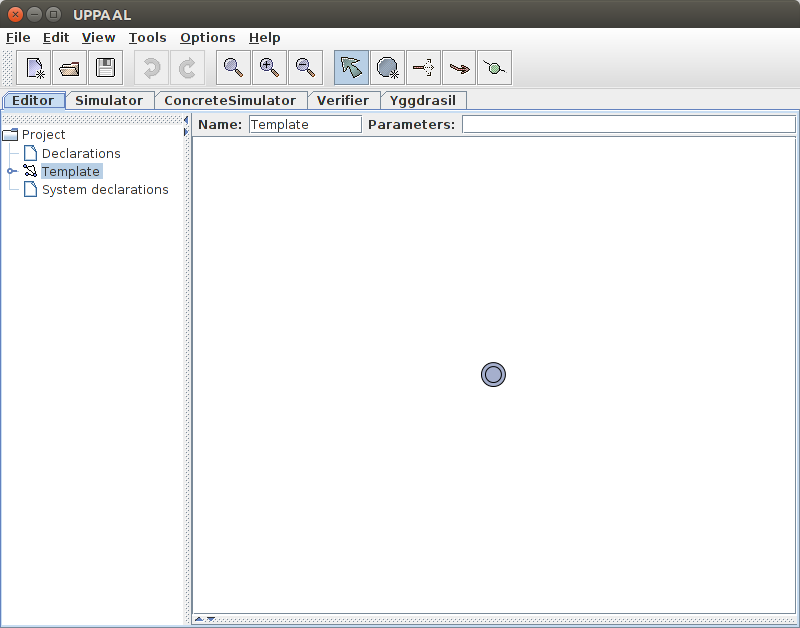
\includegraphics[width=0.6\textwidth]{images/UPPAAL_window}
% \end{center}
% \caption{\label{fig:uppaal-window}The main window of UPPAAL.}
% \end{figure}


\subsection{Installing ANIMO}\label{sec:install-animo}
\begin{enumerate}
\item ANIMO is {\bfseries free only for academic use}. For commercial licenses, please contact us at \contactemail.
\item Run Cytoscape.
\item Click the menu command \emph{Apps} $\rightarrow$ \emph{App Manager}: the \emph{App Manager}
window will open.
\item Click on \emph{ANIMO} in the list of available apps and then on the \emph{Install} button.
 ANIMO will be automatically downloaded and installed.
\item You can close the \emph{App Manager} window.
\item ANIMO will automatically try to locate the \emph{verifyta} executable included in UPPAAL, which is needed to verify Timed Automata models.
If you know the location where you installed UPPAAL, you can just stop the process (press on the small {\tt X} on the right), and indicate the
location of the \emph{verifyta} executable.
You can find it 
\macpc{where it was copied at step~\ref{step:mac-install-uppaal} in Section~\ref{sec:install-uppaal}}{in the \emph{bin} (\emph{bin-Linux}, \emph{bin-Win32},
\dots\ depending on your operating system)
directory inside the UPPAAL installation directory, where it was unzipped at step~\ref{step:unzip-uppaal} in Section~\ref{sec:install-uppaal}}
\item ANIMO is correctly installed and ready to be used.
\end{enumerate}

\clearpage
\section{ANIMO user's manual}\label{sec:animo-manual}
We will now present a step-by-step sequence to obtain an example model
with ANIMO, which will allow us to illustrate the main features of the tool.

\subsection{Modelling a small network}\label{sec:modeling-network-example}
\begin{enumerate}
\item Run Cytoscape.
\item If Cytoscape is already running and there are open documents, please make sure that the current work is saved before proceeding.
\item From the \emph{File} menu, select \emph{New} $\rightarrow$ \emph{Session}. Answer positively to the question
``\emph{Current session (all networks/attributes) will be lost. Do you want to continue?}''.
\item From the \emph{File} menu, select \emph{New} $\rightarrow$ \emph{Network} $\rightarrow$ \emph{Empty Network}.
\item Click \emph{OK} in the \emph{Create New Network} dialogue. A new white window will open: there we will insert the nodes for the new network.
\item\label{step:add-nodes} Add $5$ nodes to the empty network by right-clicking
on empty areas of the \emph{Network} window, and selecting \emph{Add} $\rightarrow$ \emph{Node}.\\
\emph{Note}: \emph{right-clicks} are available only on mice with at least two buttons. On Apple mice,
or devices with only one button, it is necessary to keep the button with the \maccmd\ symbol (or possibly Ctrl) pressed while clicking.
\item The \emph{Edit reactant} dialogue window is opened every time a new node is added,
or when you right click an existing node and then select the \emph{ANIMO} $\rightarrow$ \emph{Edit reactant\dots}
item from the menu, or when you double-click on an existing node.
Use that window to set the properties of the nodes as indicated in Table~\ref{tab:setting-nodes},
taking the setting in Figure~\ref{fig:edit-reactant} for node A as reference. When
the properties of a node have been inserted, confirm the choice with the \emph{Save} button.
\newcounter{miocounterperenumerate}
\setcounter{miocounterperenumerate}{\value{enumi}}
\end{enumerate}\vspace{-2ex}

\begin{table}[htbp]
\begin{minipage}{\textwidth}
\begin{center}
\caption{The settings for the nodes (signalling network components) in the example.\label{tab:setting-nodes}}
{\begin{tabular}{llllll}%|c|c|c|c|c|c|}
\ \\
\hline\noalign{\vskip 2mm}
  \multirow{2}{*}{{\bfseries Name}} & {\bfseries Total act.} & {\bfseries Initial act.} & \multirow{2}{*}{{\bfseries Molecule type}} &
\multirow{2}{*}{{\bfseries Enabled?}} & \multirow{2}{*}{{\bfseries Plotted?}}\\
& {\bfseries levels} & {\bfseries level} & & & \\[2mm]
\hline\noalign{\vskip 2mm}
  A & 15 & 15 & Cytokine & Yes & No\\[5mm]
  B & 15 & 0 & Receptor & Yes & No\\[5mm]
  C & 15 & 0 & Other & Yes & No\\[5mm]
  D & 100 & 0 & Kinase & Yes & Yes\\[5mm]
  E & 1 & 1 & Phosphatase & Yes & No\\[2mm]
\hline
\end{tabular}
}{}
\end{center}
\end{minipage}
\end{table}

\begin{figure}[htpb]
\begin{minipage}{\textwidth}
\begin{center}
 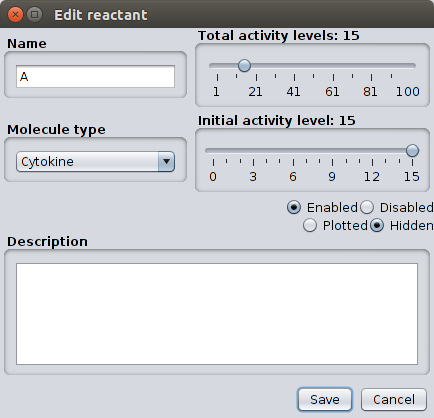
\includegraphics[width=.45\textwidth]{images/edit_reactantA_new}\\
 \caption{The \emph{Edit reactant} window: modifying the properties of node A. The \emph{Description}
box in the \emph{Edit reactant} dialogue can be used to add comments about what a node represents or where its reference was found in literature:
when keeping the mouse cursor over that node in the network, the description text will be shown as tool-tip.}\label{fig:edit-reactant}
\end{center}
\end{minipage}
\end{figure}


\begin{enumerate}
\setcounter{enumi}{\value{miocounterperenumerate}}
\item\label{step:add-edges} In order to add an edge to the network, right-click on the node from which the
edge should start, select \emph{Add} $\rightarrow$ \emph{Edge}, and click on the node where the edge should arrive.
Add the following edges: A~$\rightarrow$~B, B~$\rightarrow$~C,
C~$\rightarrow$~B, B~$\rightarrow$~D, E~$\rightarrow$~D.
\item The \emph{Edit interaction} dialogue window is opened when you add a new edge,
or when you right click an existing edge and then select the \emph{ANIMO} $\rightarrow$ \emph{Edit interaction\dots} item
from the menu, or when you double-click on an existing edge.
Use that window to set the parameters of the edges as indicated in Table~\ref{tab:setting-edges}. The settings
for the edge A $\rightarrow$ B should reflect the ones shown in the \emph{Interaction A $\rightarrow$ B} window in Figure~\ref{fig:edit-reaction}.\\
\emph{Note}: In order to insert a qualitative parameter like the ones required by the example network,
click once the slider in the \emph{parameter} box to activate it, and then move the slider to match the requested value.
\setcounter{miocounterperenumerate}{\value{enumi}}
\end{enumerate}

\begin{table}[!ht]
\begin{minipage}{\textwidth}
\begin{center}
\caption{The settings for the edges (interactions) in the example.\label{tab:setting-edges}}
{\begin{tabular}{llll}%|c|c|c|c|}
\ \\
\hline\noalign{\vskip 2mm}
  {\bfseries Interaction} & {\bfseries Influence} & {\bfseries Scenario} & {\bfseries Parameter value}\\[2mm]
\hline
\noalign{\vskip 2mm}  A $\rightarrow$ B & Activation & 1 & Medium \\[5mm]
\noalign{\vskip 2mm}  B $\rightarrow$ C & Activation & 1 & Slow \\[5mm]
\noalign{\vskip 2mm}  C $\rightarrow$ B & Inhibition & 1 & Fast \\[5mm]
\noalign{\vskip 2mm}  B $\rightarrow$ D & Activation & 1 & Slow \\[5mm]
\noalign{\vskip 2mm}  E $\rightarrow$ D & Inhibition & 2 & V. Slow \\[2mm]
\hline
\end{tabular}}{}
\end{center}
\end{minipage}
\end{table}\vspace{-2ex}

\begin{figure}[!tpb]
\begin{minipage}{\textwidth}
\begin{center}
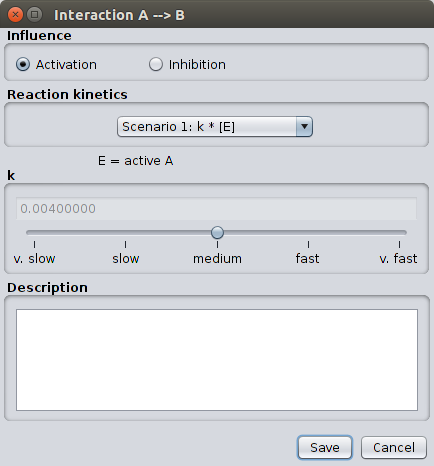
\includegraphics[width=.45\textwidth]{images/edit_reactionAB_new}\\
\caption{The \emph{Edit interaction} window: modifying the properties of edge A $\rightarrow$ B. There is a
\emph{Description} box also for interactions: it can be used with the same aim as for nodes.}\label{fig:edit-reaction}
\end{center}
\end{minipage}
\end{figure}

\begin{enumerate}
\setcounter{enumi}{\value{miocounterperenumerate}}
\item In the \emph{Control Panel}, make sure that the \emph{ANIMO} tab is selected by clicking its title.
\item Insert a value of {\tt 120} minutes in the \emph{Simulation} box.
\item Click the \emph{Analyse network} button (alternatively, you can press Return after inserting the number of minutes).
\item After a few seconds the \emph{Results Panel} should appear on the right,
showing a plot of the activity level of reactant D over a time course of 120 minutes.
Figure~\ref{fig:rete-esempio} shows the resulting network and graph plot.
\end{enumerate}

\begin{figure}[!tpb]
\begin{minipage}{\textwidth}
\begin{center}
  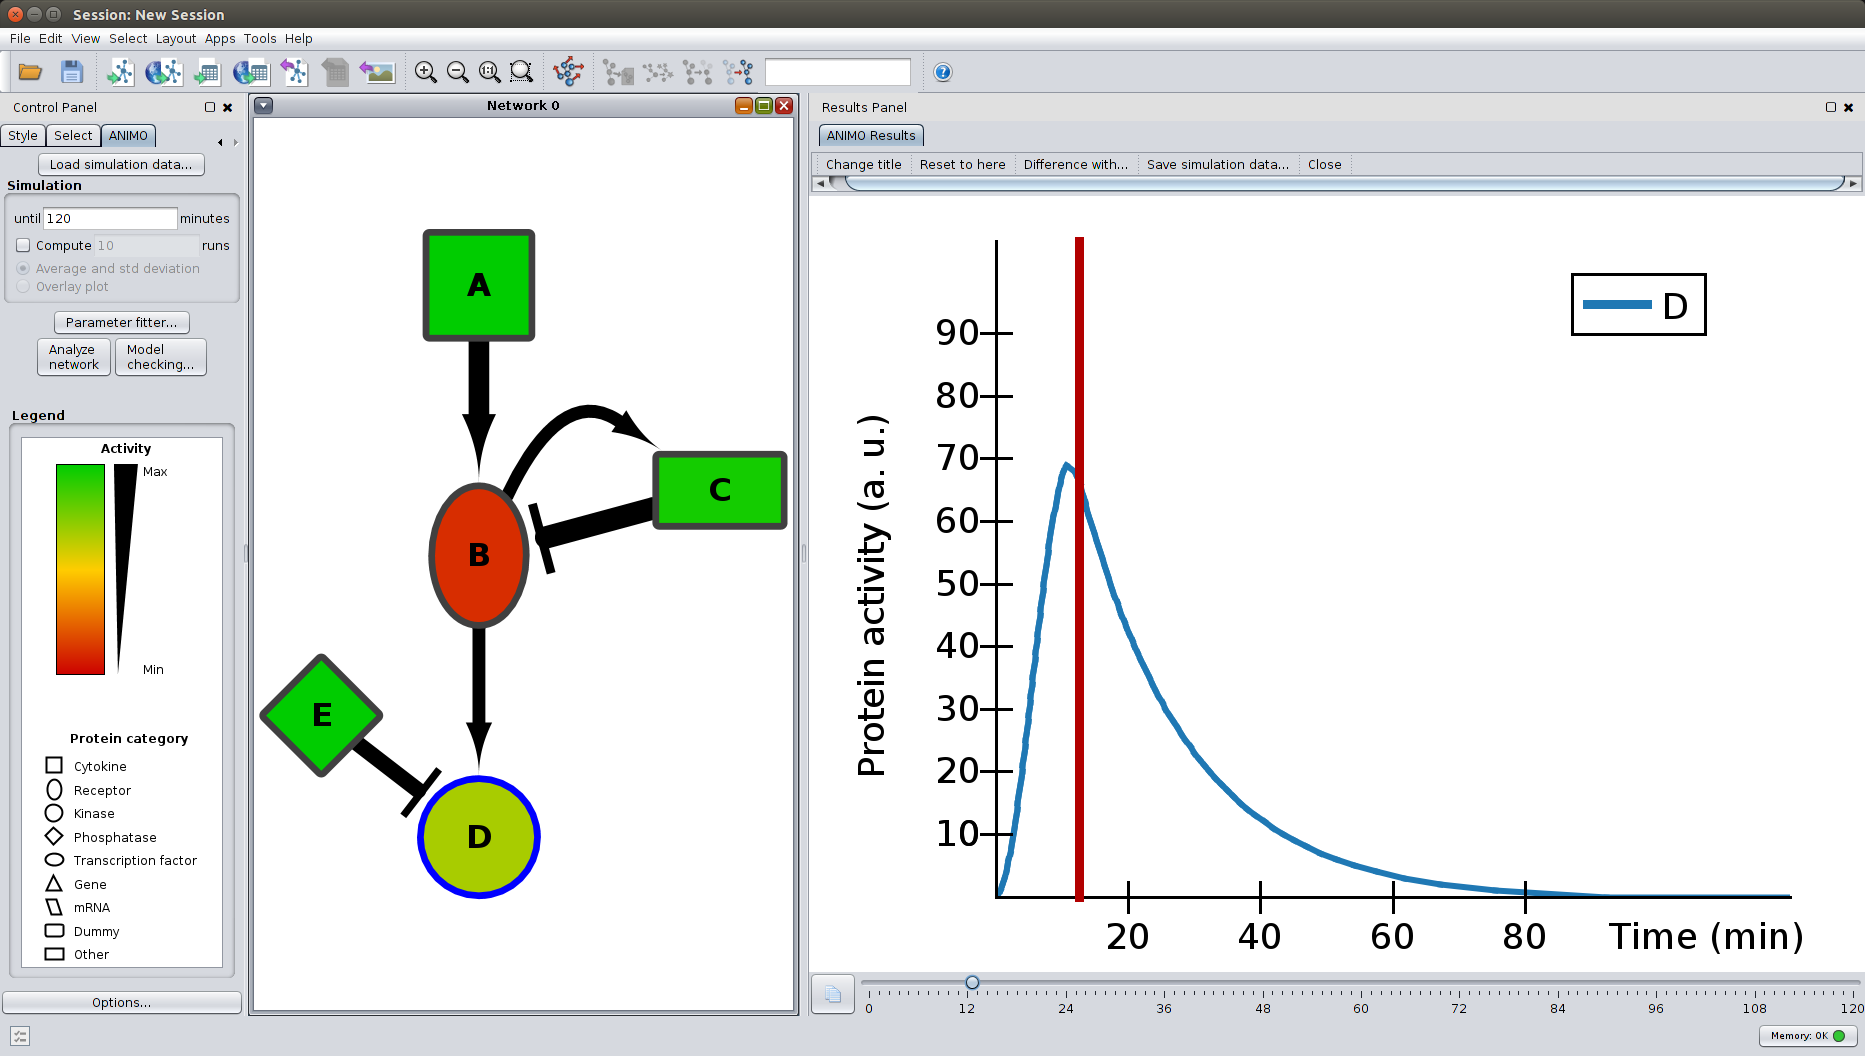
\includegraphics[width=.9\textheight, angle=90]{images/esempio_uso_ANIMO_new}
\end{center}
\caption{The completed example, where also the feature that allows to view the activity levels
of reactants at chosen simulation times is demonstrated: the vertical red bar in the graph on the
right can be moved through the slider under the graph, and indicates the point in the time series
on which the colouring of the nodes in the \emph{Network} window is based.
The legends for colours and shapes can be found in the \emph{Legend} panel.}\label{fig:rete-esempio}
\end{minipage}
\end{figure}


\subsubsection{Managing simulation data and activity levels plots}
Each time a simulation result is obtained, a new tab is added to the \emph{Results Panel} (see the right part of Fig.~\ref{fig:rete-esempio})
in which we identify a set of buttons, a plot of the activity levels of the selected reactants and a time slider.

The buttons above the graph have the following purposes:
\begin{description}
  \item[Change title] allows to select a new title for the tab: this can be useful e.g. when comparing different
simulations made on similar configurations of the same network
  \item[Reset to here] restore the network to the state it was in when the simulation that gave the current graph was performed.
If no simulation was done with the network in its current state, the current network configuration will be lost
  \item[Difference with\dots] allows to compute a difference between two simulations. After pressing this button, select another
graph (i.e. another tab in the \emph{Results} panel) and click on the \emph{Difference with this} button: a new graph will be shown,
highlighting the differences between the two selected graphs (first - second)
  \item[Save simulation data\dots] allows to save
the simulation data of the current tab on a \emph{.sim} file, which can then be loaded and inspected in the future.
The \emph{Load simulation data\dots} button in the \emph{Control Panel} above the \emph{Simulation} box can be used for this purpose.
Please note that the best results are obtained only when loading a \emph{.sim} file when the \emph{Network} window contains the same network
on which the simulation data are based. If no network is currently opened, a network will \emph{not} be opened by loading a \emph{.sim} file.
  \item[Close] close the currently displayed graph.
\end{description}


Right clicking inside the graph area will bring up a menu that allows to perform some basic operations with the graph
and its data:
\begin{itemize}
  \item \emph{Add data from CSV}: \label{csv-import-format}superpose the graph with other data series found in a \emph{.csv} (comma separated values) file. This file type can be
obtained for example by exporting data from the default Excel format. If you want the data in the \emph{.csv} file to be rescaled so
that its maximum Y value coincides with the maximum in the plot, the data file needs to contain a column named (exactly)
\emph{Number\_{}of\_{}levels}, on the first row of which the maximum of the scale for the \emph{.csv} data needs to be put. For example,
if the data in the \emph{.csv} file are on a 0-100 scale, the value for \emph{Number\_{}of\_{}levels} will be 100.
  \item \emph{Save as PNG}: save the graph as it is shown in a \emph{.png} image file. This file format can be opened by most
image editors.
  \item \emph{Export visible as CSV}: export to a \emph{.csv} file all the series that are currently visible (i.e., not hidden)
in the graph.
  \item \emph{Clear Data}: clear the contents of the graph, removing all series. This can be useful for plotting
a \emph{.csv} file without superposing it to the current graph, or for loading a file in which all hidden data where removed
(exporting the visible graph to a \emph{.csv} with the previous command).
  \item \emph{Graph interval}: change the lower and upper bounds for X and Y axes.
  \item \emph{Zoom rectangle}: zoom the graph around a user-chosen rectangular area.
    After selecting this command the shape of the mouse cursor changes into a cross. The area of the plot to be
    zoomed can then be selected by dragging a rectangular selection around it (see the definition of \emph{rectangular
    selection} on page~\pageref{nota:rectangular-selection}).
  \item \emph{Zoom extents}: bring the zoom level back to default, cancelling the effects of any \emph{Zoom rectangle}
command.
\end{itemize}

Whenever the result of one or more simulations is shown as a graph, it is possible to use the slider under the graph to
move through the entire simulation, showing the activity levels of all reactants represented with different node colouring in
the \emph{Network} window on the left. For an example, see Figure~\ref{fig:rete-esempio}: the vertical red line in the
graph represents the time instant on which the colours of the nodes in the \emph{Network} window are based, and can
be moved with the slider over which the mouse cursor is drawn.

Finally, the \emph{Copy} button beside the slider can be used to set the activity levels in the network to the time point
selected with the slider. This is useful if for example we want to change some conditions from a certain point in a simulation.



% \subsection{Additional tips}
\subsubsection{Editing a network in Cytoscape}
Nodes and arcs can be placed in the network as shown previously: right click on an empty space
in the \emph{Network} window and select \emph{Add} $\rightarrow$ \emph{Node} to add a node;
right click on the source node and select \emph{Add} $\rightarrow$ \emph{Edge}, then click on
the target node to create a new edge between the two nodes.

In order to delete a node/edge, select them by clicking
or grouping them in a larger rectangular selection, and then press the \emph{Delete} key on the keyboard
or select the \emph{Edit} $\rightarrow$ \emph{Delete Selected Nodes and Edges} menu command.\\
\emph{Note}: in order to obtain a \emph{rectangular selection}\label{nota:rectangular-selection},
left click in the \emph{Network} window where the upper-left corner of the rectangle should be and,
without releasing the left mouse button, drag the mouse cursor to where the lower-right corner of the
rectangular selection should be; then release the left mouse button. All the entities which were
\emph{even partially} touched by the rectangle are now selected.

Navigation inside the \emph{Network} window can be performed by clicking and dragging the centre mouse button,
while zooming can be done by either rotating the mouse wheel or clicking and holding the right mouse button
while moving the mouse in a vertical direction. In case no central mouse button is available, the \emph{Network}
tab in the \emph{Control Panel} will allow to navigate the network, together with the zoom buttons available in
Cytoscape's toolbar (where the open and save icons are).

Finally, note that the colours used to represent node activity can be changed using the \emph{Style} tab
in the \emph{Control Panel}. Please refer to Cytoscape's manual to do that.
% interface provided by Cytoscape, changing the setting for \emph{Node colour}, shown in Figure~\ref{fig:change-gradient}.
% To change the node colours, activate the \emph{VizMapper\texttrademark} tab in the \emph{Control Panel}, and
% find the entry named \emph{Node Colour} in the \emph{Visual Mapping Browser} box. Click the arrow-shaped
% icon directly to the left of \emph{Node Colour}: the current setting for the node colours should appear:
% click the coloured bar to open the window shown in Figure~\ref{fig:change-gradient}.
% The \emph{activityRatio} on which the node colouring is based is the ratio between the current activity level
% of a node and its number of activity levels.
% The coloured arrows pointing downward on the upper border of the coloured rectangle can be dragged along the length of the $[0, 1]$
% interval, thus changing the point at which a particular colour appears. New arrows can be added with the \emph{Add} button, while
% clicking an arrow and pressing the \emph{Delete} button will remove one. To change the colour of a point in the interval,
% double click the corresponding arrow, and a new window will open, allowing you to choose a new colour: clicking \emph{OK} will
% accept the new colour. The modifications made in the \emph{Gradient Editor for Node Colour} window should be automatically reflected in
% the model: when the gradient is as wanted, simply close the window. If the node colours seem not to have been updated, please move the
% slider under an existing graph in the \emph{Results Panel}.
% 
% \begin{figure}[!tpb]
% \begin{minipage}{\textwidth}
% \centering
%   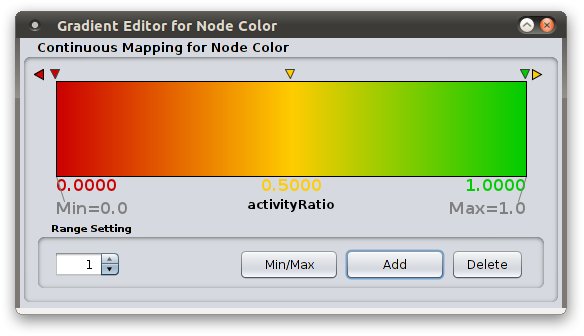
\includegraphics[width=.6\textwidth]{images/editing-gradient2}
%   \caption{Changing the colours used to represent node activity in an ANIMO model.}\label{fig:change-gradient}
% \end{minipage}
% \end{figure}


\subsection{ANIMO features}
Nodes and edges (and groups of nodes/edges highlighted via a rectangular selection)
can be disabled by choosing \emph{ANIMO} $\rightarrow$ \emph{Enable/disable} from
the right-click menu: they will be represented with less saturated colours and can be re-enabled by performing
the same action. Moreover, a node can be enabled/disabled directly in its properties window, where it is
also possible to add/remove the node from the list of series appearing in the graph resulting from a simulation
of the network by selecting \emph{Plotted} or \emph{Hidden} (see also Figure~\ref{fig:edit-reactant}):
nodes that will be plotted have a blue border.
Every enabled node will be taken into account when computing the evolution of the system,
but only nodes marked as \emph{Plotted} will appear in a graph.

Each plot in an \emph{ANIMO Results} tab contains by default a legend, which can be used to modify which series are
displayed and how they are displayed. Clicking with the central mouse button on a series name will hide it from the
graph, while a centre-click on the coloured line beside the series name will change the colour of that series,
cycling through a predefined set of available colours. The entire legend can be hidden by clicking with the
central mouse button anywhere on the graph (not inside the legend), or it can be dragged around by clicking and holding the left
mouse button, releasing it when the preferred position is reached. Rotating the mouse wheel will allow the thickness of all
the graph lines, and the size of the text, to grow or decrease: this feature can be useful when the window containing
the graph is very large.

If the model is non-deterministic, i.e. its
evolution is not expected to be exactly the same for every single simulation run (see the uncertainty settings in Options, Section~\ref{sec:animo-options}),
it is possible to ask ANIMO to perform
a number of simulation runs in a batch, plotting the averages of the activity levels over the runs together with a standard
deviation value, or showing a so-called \emph{overlay plot} where all runs are plotted over each other. The controls
that allow to ask for multiple simulation runs can be found in the \emph{Control Panel}, inside the \emph{Simulation} box.

Standard deviation may be represented in the graph: it is normally shown as vertical bars, but its aspect can be
cycled through five possibilities (vertical bars, shading, both bars and shading, bars and symbols, none) by right-clicking the
corresponding line in the legend. Symbols associated to a representation of standard deviation can be changed by Shift-right-clicking
(holding down the \emph{Shift} key, right click) on the corresponding line in the legend.
Standard deviation values can be obtained when asking for multiple simulations in the network
analysis, but they can also be present in a \emph{.csv} file, e.g. when the file contains averages of (replicated) experimental data.
In a \emph{.csv} file, the column containing the standard deviation values for column \emph{A}
should be named \emph{A\_{}StdDev} for ANIMO to recognize it and properly display the data series
with the associated error values.



\subsection{Parameter settings}
The application of some basic strategies when setting the parameters for a network allows
the less experienced users to considerably shorten the modelling time.
First of all, it is important to proceed in a \emph{top-to-bottom} order, trying to match
a component to the corresponding data before inserting the components downstream thereof.
Second, when choosing the kinetic parameter for an interaction, we advise to first use the qualitative settings (very slow, slow, medium, fast, very fast):
this allows to define the relative speeds of the interactions as soon as possible,
leaving the more precise parameter setting procedure as a follow-up step. Finally, as can be seen from
the parameter settings of Section~\ref{sec:modeling-network-example}, in order to obtain a peak
behaviour it is particularly important that
a negative feedback is present (as an example, see the interactions involving B and C in Tab.~\ref{tab:setting-edges}),
and that the inactivating interaction in the loop is faster than the ones activating the target node.

Once a satisfying profile is obtained, the parameters can be rescaled in groups or all at the same time.
This allows us to easily match a model against experimental data that show a similar profile on a different
time scale (e.g., the model produces a peak similar to the one in the data, but 20 minutes too early).
In order to rescale a set of reactions, select the corresponding edges in the \emph{Network} window,
right click on one of the selected edges and choose \emph{ANIMO} $\rightarrow$ \emph{Rescale k value(s)}
from the menu. In the new dialogue, insert the scale factor that will be applied to the selected reactions and
press \emph{OK}: the new values will be automatically computed and set by ANIMO.

% A final note on the \emph{seconds/step} button. This button allows to define the time granularity
% of the simulations, but it is not strictly necessary to choose a very precise value.
% % As the time bounds in the \tas\ model are integers, rounding errors can make the model
% % behave differently from what the parameters define.
% If the current value for \emph{seconds/step}
% is too high (or too low) to allow the network to be properly simulated, ANIMO will automatically choose (respectively)
% the highest (lowest) value that still allows to avoid rounding problems. It will be possible to notice
% such a change in the value of time scale when the number on the \emph{seconds/step} button changes.


\subsection{Opening a Timed Automata model generated by ANIMO}
All Timed Automata models generated by ANIMO in a Cytoscape session are available
until Cytoscape is closed, and can be usually found in the system temporary directory.
In order to know exactly where the Timed Automata model for a particular simulation
was saved, check the Cytoscape log (small button on the lower-left-most corner in Cytoscape):
it contains the advancement status of all the executed tasks, including ANIMO simulations.
Before beginning the analysis, each simulation task explicitly outputs the location
of the file that is going to be analysed. Opening the same file with UPPAAL will allow
the interested user to inspect the model by themselves, and query it for other properties
directly in the UPPAAL user interface.


\subsection{Updating ANIMO}
To check whether a new version of ANIMO has been published, run Cytoscape and open
the app manager via the menu command \emph{Apps} $\rightarrow$ \emph{App Manager}.
In the \emph{Check for Updates} tab the available updates will be listed:
if a new version of ANIMO was published, it will appear in the table. Select it
and press \emph{Updated Selected}, or just press \emph{Update All} to update all apps.
Cytoscape will download and install the new versions of the apps.

\subsection{ANIMO Options}\label{sec:animo-options}
In the \emph{Control Panel}, the \emph{ANIMO} tab contains also an \emph{Options\dots} button:
it is located below the \emph{Legend}. Pressing that button will open the options dialogue for
ANIMO, where the following configuration settings can be changed:
\begin{description}
  \item[location of the \emph{verifyta} executable]: the location of \emph{verifyta}
    can be changed if for example a wrong location was previously selected,
    UPPAAL was not already installed when ANIMO was run for the first time, or a new
    version of UPPAAL was installed
  \item[uncertainty in reaction parameters]: a degree of uncertainty can be set for the
    $k$ parameters of all the reactions in ANIMO models, introducing some non-determinism
    in the simulations. For example, if a value of 5\% uncertainty is chosen, a given reaction
    that would normally take exactly 10 seconds to perform will occur after a number of
    seconds randomly chosen from a uniform distribution in the closed interval $9.95, 10.05$.
    The default value for uncertainty is 5, so reaction times are as described by default.
    In order to get a deterministic model (especially useful to make model checking much
    easier for the computer), set this parameter to 0, i.e. uncheck the option.
  \item[type of underlying Timed Automata model]: two types of Timed Automata models are
    available: reaction-centred and reactant-centred. The latter is in general more efficient
    and is selected by default. The difference between the two models can be seen by opening
    the models generated by ANIMO when each choice is made.
\end{description}




\end{document}